\documentclass[14pt,russian]{extarticle}		
\usepackage{lmodern}
\usepackage{float}
\usepackage{xcolor}
\usepackage{subfig}
\usepackage[export]{adjustbox}

\usepackage{setspace}
\onehalfspacing % полуторный интервал

%%%%%%%%%%%%%%%%%%%%%%%
%%% Проверка используемого TeX-движка %%%
\usepackage{iftex}
\newif\ifxetexorluatex   % определяем новый условный оператор (http://tex.stackexchange.com/a/47579/79756)
\ifXeTeX
    \xetexorluatextrue
\else
    \ifLuaTeX
        \xetexorluatextrue
    \else
        \xetexorluatexfalse
    \fi
\fi

%%% Поля и разметка страницы %%%
\usepackage{pdflscape}                              % Для включения альбомных страниц
\usepackage{geometry}                               % Для последующего задания полей
\geometry{a4paper,tmargin=2cm,bmargin=2cm,lmargin=3cm,rmargin=1cm} % тоже самое, но лучше

%%% Математические пакеты %%%
\usepackage{amsthm,amsfonts,amsmath,amssymb,amscd}  % Математические дополнения от AMS
\usepackage{mathtools}                              % Добавляет окружение multlined

%%%% Установки для размера шрифта 14 pt %%%%
%% Формирование переменных и констант для сравнения (один раз для всех подключаемых файлов)%%
%% должно располагаться до вызова пакета fontspec или polyglossia, потому что они сбивают его работу
\newlength{\curtextsize}
\newlength{\bigtextsize}
\setlength{\bigtextsize}{13.9pt}

\makeatletter
%\show\f@size                                       % неплохо для отслеживания, но вызывает стопорение процесса, если документ компилируется без команды  -interaction=nonstopmode 
\setlength{\curtextsize}{\f@size pt}
\makeatother

%%% Кодировки и шрифты %%%
\ifxetexorluatex
    \usepackage{polyglossia}                        % Поддержка многоязычности (fontspec подгружается автоматически)
\else
    \RequirePDFTeX                                  % tests for PDFTEX use and throws an error if a different engine is being used
   %%% Решение проблемы копирования текста в буфер кракозябрами
%    \input glyphtounicode.tex
%    \input glyphtounicode-cmr.tex %from pdfx package
%    \pdfgentounicode=1
    \usepackage{cmap}                               % Улучшенный поиск русских слов в полученном pdf-файле
    \defaulthyphenchar=127                          % Если стоит до fontenc, то переносы не впишутся в выделяемый текст при копировании его в буфер обмена
    \usepackage[T2A]{fontenc}                       % Поддержка русских букв
    \usepackage[utf8]{inputenc}                     % Кодировка utf8
    \usepackage[english, russian]{babel}            % Языки: русский, английский
    \IfFileExists{pscyr.sty}{\usepackage{pscyr}}{}  % Красивые русские шрифты
\fi

%%% Оформление абзацев %%%
\usepackage{indentfirst}                            % Красная строка

%%% Таблицы %%%
\usepackage{longtable}                              % Длинные таблицы
\usepackage{multirow,makecell,array}                % Улучшенное форматирование таблиц
\usepackage{booktabs}                               % Возможность оформления таблиц в классическом книжном стиле (при правильном использовании не противоречит ГОСТ)

%%% Общее форматирование
\usepackage{soulutf8}                               % Поддержка переносоустойчивых подчёркиваний и зачёркиваний
\usepackage{icomma}                                 % Запятая в десятичных дробях


%%% Гиперссылки %%%
\usepackage{hyperref}

%%% Изображения %%%
\usepackage{graphicx}                               % Подключаем пакет работы с графикой

%%% Списки %%%
\usepackage{enumitem}

%%% Подписи %%%
\usepackage{caption}                                % Для управления подписями (рисунков и таблиц) % Может управлять номерами рисунков и таблиц с caption %Иногда может управлять заголовками в списках рисунков и таблиц

%%% Интервалы %%%

%%% Счётчики %%%
\usepackage[figure,table]{totalcount}               % Счётчик рисунков и таблиц
\usepackage{totcount}                               % Пакет создания счётчиков на основе последнего номера подсчитываемого элемента (может требовать дважды компилировать документ)
\usepackage{totpages}                               % Счётчик страниц, совместимый с hyperref (ссылается на номер последней страницы). Желательно ставить последним пакетом в преамбуле

%%% Продвинутое управление групповыми ссылками (пока только формулами) %%%
\ifxetexorluatex
    \usepackage{cleveref}                           % cleveref корректно считывает язык из настроек polyglossia
\else
    \usepackage[russian]{cleveref}                  % cleveref имеет сложности со считыванием языка из babel. Такое решение русификации вывода выбрано вместо определения в documentclass из опасности что-то лишнее передать во все остальные пакеты, включая библиографию.
\fi
\creflabelformat{equation}{#2#1#3}                  % Формат по умолч  
%%% Кодировки и шрифты %%%
\ifxetexorluatex
    \setmainlanguage[babelshorthands=true]{russian}  % Язык по-умолчанию русский с поддержкой приятных команд пакета babel
    \setotherlanguage{english}                       % Дополнительный язык = английский (в американской вариации по-умолчанию)
    \ifXeTeX
        \defaultfontfeatures{Ligatures=TeX,Mapping=tex-text}
    \else
        \defaultfontfeatures{Ligatures=TeX}
    \fi
	\setmainfont{Times New Roman}
	\newfontfamily\cyrillicfont{Times New Roman}
	\setsansfont{Times New Roman}                    %% задаёт шрифт без засечек
	\setmonofont{Liberation Mono}               %% задаёт моноширинный шрифт
\else
    \IfFileExists{pscyr.sty}{\renewcommand{\rmdefault}{ftm}}{}
\fi

%%% Интервалы %%%
%linespread-реализация ближе к реализации полуторного интервала в ворде.
%setspace реализация заточена под шрифты 10, 11, 12pt, под остальные кегли хуже, но всё же ближе к типографской классике. 
%\linespread{1.3}                    % Полуторный интервал (ГОСТ Р 7.0.11-2011, 5.3.6)

%%% Выравнивание и переносы %%%
\sloppy                             % Избавляемся от переполнений
\clubpenalty=10000                  % Запрещаем разрыв страницы после первой строки абзаца
\widowpenalty=10000                 % Запрещаем разрыв страницы после последней строки абзаца

%%% Подписи %%%
\captionsetup{%
singlelinecheck=off,                % Многострочные подписи, например у таблиц
skip=2pt,                           % Вертикальная отбивка между подписью и содержимым рисунка или таблицы определяется ключом
justification=centering,            % Центрирование подписей, заданных командой \caption
}
%%%        Подключение пакетов                 %%%
\usepackage{ifthen}                 % добавляет ifthenelse
%%% Инициализирование переменных, не трогать!  %%%
\newcounter{intvl}
\newcounter{otstup}
\newcounter{contnumeq}
\newcounter{contnumfig}
\newcounter{contnumtab}
\newcounter{pgnum}
\newcounter{bibliosel}
\newcounter{chapstyle}
\newcounter{headingdelim}
\newcounter{headingalign}
\newcounter{headingsize}
\newcounter{tabcap}
\newcounter{tablaba}
\newcounter{tabtita}
%%%%%%%%%%%%%%%%%%%%%%%%%%%%%%%%%%%%%%%%%%%%%%%%%%

%%% Область упрощённого управления оформлением %%%

%% Интервал между заголовками и между заголовком и текстом
% Заголовки отделяют от текста сверху и снизу тремя интервалами (ГОСТ Р 7.0.11-2011, 5.3.5)
\setcounter{intvl}{3}               % Коэффициент кратности к размеру шрифта

%% Отступы у заголовков в тексте
\setcounter{otstup}{0}              % 0 --- без отступа; 1 --- абзацный отступ

%% Нумерация формул, таблиц и рисунков
\setcounter{contnumeq}{1}           % Нумерация формул: 0 --- пораздельно (во введении подряд, без номера раздела); 1 --- сквозная нумерация по всей диссертации
\setcounter{contnumfig}{1}          % Нумерация рисунков: 0 --- пораздельно (во введении подряд, без номера раздела); 1 --- сквозная нумерация по всей диссертации
\setcounter{contnumtab}{1}          % Нумерация таблиц: 0 --- пораздельно (во введении подряд, без номера раздела); 1 --- сквозная нумерация по всей диссертации

%% Оглавление
\setcounter{pgnum}{0}               % 0 --- номера страниц никак не обозначены; 1 --- Стр. над номерами страниц (дважды компилировать после изменения)

%% Библиография
\setcounter{bibliosel}{1}           % 0 --- встроенная реализация с загрузкой файла через движок bibtex8; 1 --- реализация пакетом biblatex через движок biber

%% Текст и форматирование заголовков
\setcounter{chapstyle}{1}           % 0 --- разделы только под номером; 1 --- разделы с названием "Глава" перед номером
\setcounter{headingdelim}{1}        % 0 --- номер отделен пропуском в 1em или \quad; 1 --- номера разделов и приложений отделены точкой с пробелом, подразделы пропуском без точки; 2 --- номера разделов, подразделов и приложений отделены точкой с пробелом.

%% Выравнивание заголовков в тексте
\setcounter{headingalign}{0}        % 0 --- по центру; 1 --- по левому краю

%% Размеры заголовков в тексте
\setcounter{headingsize}{0}         % 0 --- по ГОСТ, все всегда 14 пт; 1 --- пропорционально изменяющийся размер в зависимости от базового шрифта

%% Подпись таблиц
\setcounter{tabcap}{0}              % 0 --- по ГОСТ, номер таблицы и название разделены тире, выровнены по левому краю, при необходимости на нескольких строках; 1 --- подпись таблицы не по ГОСТ, на двух и более строках, дальнейшие настройки: 
%Выравнивание первой строки, с подписью и номером
\setcounter{tablaba}{2}             % 0 --- по левому краю; 1 --- по центру; 2 --- по правому краю
%Выравнивание строк с самим названием таблицы
\setcounter{tabtita}{1}             % 0 --- по левому краю; 1 --- по центру; 2 --- по правому краю

%%% Рисунки %%%
\DeclareCaptionLabelSeparator*{emdash}{~--- }             % (ГОСТ 2.105, 4.3.1)
\captionsetup[figure]{labelsep=emdash,font=onehalfspacing,position=bottom}

%%% Таблицы %%%
\ifthenelse{\equal{\thetabcap}{0}}{%
    \newcommand{\tabcapalign}{\raggedright}  % по левому краю страницы или аналога parbox
}

\ifthenelse{\equal{\thetablaba}{0} \AND \equal{\thetabcap}{1}}{%
    \newcommand{\tabcapalign}{\raggedright}  % по левому краю страницы или аналога parbox
}

\ifthenelse{\equal{\thetablaba}{1} \AND \equal{\thetabcap}{1}}{%
    \newcommand{\tabcapalign}{\centering}    % по центру страницы или аналога parbox
}

\ifthenelse{\equal{\thetablaba}{2} \AND \equal{\thetabcap}{1}}{%
    \newcommand{\tabcapalign}{\raggedleft}   % по правому краю страницы или аналога parbox
}

\ifthenelse{\equal{\thetabtita}{0} \AND \equal{\thetabcap}{1}}{%
    \newcommand{\tabtitalign}{\raggedright}  % по левому краю страницы или аналога parbox
}

\ifthenelse{\equal{\thetabtita}{1} \AND \equal{\thetabcap}{1}}{%
    \newcommand{\tabtitalign}{\centering}    % по центру страницы или аналога parbox
}

\ifthenelse{\equal{\thetabtita}{2} \AND \equal{\thetabcap}{1}}{%
    \newcommand{\tabtitalign}{\raggedleft}   % по правому краю страницы или аналога parbox
}

\DeclareCaptionFormat{tablenocaption}{\tabcapalign #1\strut}        % Наименование таблицы отсутствует
\ifthenelse{\equal{\thetabcap}{0}}{%
    \DeclareCaptionFormat{tablecaption}{\tabcapalign #1#2#3}
    \captionsetup[table]{labelsep=emdash}                       % тире как разделитель идентификатора с номером от наименования
}{%
    \DeclareCaptionFormat{tablecaption}{\tabcapalign #1#2\par%  % Идентификатор таблицы на отдельной строке
        \tabtitalign{#3}}                                       % Наименование таблицы строкой ниже
    \captionsetup[table]{labelsep=space}                        % пробельный разделитель идентификатора с номером от наименования
}
\captionsetup[table]{format=tablecaption,singlelinecheck=off,font=onehalfspacing,position=top,skip=0pt}  % многострочные наименования и прочее
\DeclareCaptionLabelFormat{continued}{Продолжение таблицы~#2}

%%% Подписи подрисунков %%%
\renewcommand{\thesubfigure}{\asbuk{subfigure}}           % Буквенные номера подрисунков
\captionsetup[subfigure]{font={normalsize},               % Шрифт подписи названий подрисунков (не отличается от основного)
    labelformat=brace,                                    % Формат обозначения подрисунка
    justification=centering,                              % Выключка подписей (форматирование), один из вариантов            
}
%\DeclareCaptionFont{font12pt}{\fontsize{12pt}{13pt}\selectfont} % объявляем шрифт 12pt для использования в подписях, тут же надо интерлиньяж объявлять, если не наследуется
%\captionsetup[subfigure]{font={font12pt}}                 % Шрифт подписи названий подрисунков (всегда 12pt)

%%% Настройки гиперссылок %%%
\ifLuaTeX
    \hypersetup{
        unicode,                % Unicode encoded PDF strings
    }
\fi

\definecolor{linkcolor}{rgb}{0.0,0,0}
\definecolor{citecolor}{rgb}{0,0.0,0}
\definecolor{urlcolor}{rgb}{0,0,0}

\hypersetup{
    linktocpage=true,           % ссылки с номера страницы в оглавлении, списке таблиц и списке рисунков
%    linktoc=all,                % both the section and page part are links
%    pdfpagelabels=false,        % set PDF page labels (true|false)
    plainpages=true,           % Forces page anchors to be named by the Arabic form  of the page number, rather than the formatted form
    colorlinks,                 % ссылки отображаются раскрашенным текстом, а не раскрашенным прямоугольником, вокруг текста
    linkcolor={linkcolor},      % цвет ссылок типа ref, eqref и подобных
    citecolor={citecolor},      % цвет ссылок-цитат
    urlcolor={urlcolor},        % цвет гиперссылок
    pdflang={ru},
}
\urlstyle{same}
%%% Шаблон %%%
\DeclareRobustCommand{\todo}{\textcolor{red}}       % решаем проблему превращения названия цвета в результате \MakeUppercase, http://tex.stackexchange.com/a/187930/79756 , \DeclareRobustCommand protects \todo from expanding inside \MakeUppercase
\setlength{\parindent}{2.5em}                       % Абзацный отступ. Должен быть одинаковым по всему тексту и равен пяти знакам (ГОСТ Р 7.0.11-2011, 5.3.7).

%%% Списки %%%
% Используем дефис для ненумерованных списков (ГОСТ 2.105-95, 4.1.7)
\renewcommand{\labelitemi}{\normalfont\bfseries{--}} 
\setlist{nosep,%                                    % Единый стиль для всех списков (пакет enumitem), без дополнительных интервалов.
    labelindent=\parindent,leftmargin=*%            % Каждый пункт, подпункт и перечисление записывают с абзацного отступа (ГОСТ 2.105-95, 4.1.8)
}
%%%%%%%%%%%%%%%%%%%%%%
\usepackage{xltxtra} % load xunicode

\usepackage{ragged2e}
\usepackage[explicit]{titlesec}
\usepackage{placeins}
\usepackage{xparse}

\usepackage{listings}
\usepackage{url} %пакеты расширений
\usepackage{algorithm, algorithmicx}
\usepackage[noend]{algpseudocode}
\usepackage{blkarray}
\usepackage{chngcntr}

  
\titleformat{name=\section,numberless}[block]{\normalfont\Large\bfseries\centering}{}{0em}{#1}
\titleformat{\section}[block]{\normalfont\Large\bfseries\raggedright}{}{0em}{\thesection\hspace{0.25em}#1}
\titleformat{\subsection}[block]{\normalfont\Large\bfseries\raggedright}{}{0em}{\thesubsection\hspace{0.25em}#1}

\let\Algorithm\algorithm
\renewcommand\algorithm[1][]{\Algorithm[#1]\setstretch{1.5}}

\usepackage{pifont}
\usepackage{calc}
\usepackage{suffix}
\usepackage{csquotes}
\DeclareQuoteStyle{russian}
    {\guillemotleft}{\guillemotright}[0.025em]
    {\quotedblbase}{\textquotedblleft}
\ExecuteQuoteOptions{style=russian}
\newcommand{\enq}[1]{\enquote{#1}}  
\newcommand{\eng}[1]{\begin{english}#1\end{english}}

\newcounter{cTheorem}
\newcounter{cDefinition}
\newcounter{cConsequent}
\newcounter{cExample}
\newcounter{cLemma}
\newtheorem{Theorem}{Теорема}[cTheorem]
\newtheorem{Definition}{Определение}[cDefinition]
\newtheorem{Consequent}{Следствие}[cConsequent]
\newtheorem{Example}{Пример}[cExample]
\newtheorem{Lemma}{Лемма}[cLemma]

\renewcommand{\theTheorem}{\arabic{Theorem}}
\renewcommand{\theDefinition}{\arabic{Definition}}
\renewcommand{\theConsequent}{\arabic{Consequent}}
\renewcommand{\theExample}{\arabic{Example}}
\renewcommand{\theLemma}{\arabic{Lemma}}
%\makeatletter
\NewDocumentCommand{\Newline}{}{\text{\\}}
\newcommand{\sequence}[2]{\ensuremath \left(#1,\ \dots,\ #2\right)}

\definecolor{mygreen}{rgb}{0,0.6,0}
\definecolor{mygray}{rgb}{0.5,0.5,0.5}
\definecolor{mymauve}{rgb}{0.58,0,0.82}
\renewcommand{\listalgorithmname}{Список алгоритмов}
\floatname{algorithm}{Листинг}
\renewcommand{\lstlistingname}{Листинг}
\renewcommand{\thealgorithm}{\arabic{algorithm}}

\newcommand{\refAlgo}[1]{(листинг \ref{#1})}
\newcommand{\refImage}[1]{(рисунок \ref{#1})}

\renewcommand{\theenumi}{\arabic{enumi}.}% Меняем везде перечисления на цифра.цифра	
\renewcommand{\labelenumi}{\arabic{enumi}.}% Меняем везде перечисления на цифра.цифра
\renewcommand{\theenumii}{\arabic{enumii}.}% Меняем везде перечисления на цифра.цифра
\renewcommand{\labelenumii}{\arabic{enumi}.\arabic{enumii}.}% Меняем везде перечисления на цифра.цифра
\renewcommand{\theenumiii}{\arabic{enumiii}.}% Меняем везде перечисления на цифра.цифра
\renewcommand{\labelenumiii}{\arabic{enumi}.\arabic{enumii}.\arabic{enumiii}.}% Меняем везде перечисления на цифра.цифра
\newfontfamily\AnkaCoder[Path=/home/nastasia/.fonts/a/]{AnkaCoder_r.ttf}
\renewcommand{\labelitemi}{--}
\renewcommand{\labelitemii}{--}

\makeatletter
\def\p@subsection{}
\def\p@subsubsection{\thesection\,\thesubsection\,}
\makeatother
\lstset{ %
  backgroundcolor=\color{white},   % choose the background color; you must add \usepackage{color} or \usepackage{xcolor}
  basicstyle=\footnotesize\AnkaCoder,        % the size of the fonts that are used for the code
  breakatwhitespace=false,         % sets if automatic breaks shoulbd only happen at whitespace
  breaklines=true,                 % sets automatic line breaking
  captionpos=top,                    % sets the caption-position to bottom
  commentstyle=\color{mygreen},    % comment style
  deletekeywords={...},            % if you want to delete keywords from the given language
  escapeinside={\%*}{*)},          % if you want to add LaTeX within your code
  extendedchars=true,              % lets you use non-ASCII characters; for 8-bits encodings only, does not work with UTF-8
  frame=single,                    % adds a frame around the code
  keepspaces=true,                 % keeps spaces in text, useful for keeping indentation of code (possibly needs columns=flexible)
  keywordstyle=\color{blue},       % keyword style
  language=python,                      % the language of the code
  morekeywords={uint64_t, uint8_t, int8_t,std,vector,uint32_t,Matrix,public,class,*,...},            % if you want to add more keywords to the set
  numbers=left,                    % where to put the line-numbers; possible values are (none, left, right)
  numbersep=5pt,                   % how far the line-numbers are from the code
  xleftmargin=25pt,
  xrightmargin=25pt,
  numberstyle=\small\color{mygray}, % the style that is used for the line-numbers
  rulecolor=\color{black},         % if not set, the frame-color may be changed on line-breaks within not-black text (e.g. comments (green here))
  showspaces=false,                % show spaces everywhere adding particular underscores; it overrides 'showstringspaces'
  showstringspaces=false,          % underline spaces within strings only
  showtabs=false,                  % show tabs within strings adding particular underscores
  stepnumber=1,                    % the step between two line-numbers. If it's 1, each line will be numbered
  stringstyle=\color{mymauve},     % string literal style
  tabsize=8,                       % sets default tabsize to 8 spaces
  title=\lstname                   % show the filename of files included with \lstinputlisting; also try caption instead of title
}
\newcommand{\anonsection}[1]{\cleardoublepage
\phantomsection
\addcontentsline{toc}{section}{\protect\numberline{}#1}
\section*{#1}}
\newcommand{\sectionbreak}{\clearpage}
\makeatletter
\let\@@scshape=\scshape
\renewcommand{\scshape}{%
  \ifnum\strcmp{\f@series}{bx}=\z@
    \usefont{T1}{cmr}{bx}{sc}%
  \else
    \ifnum\strcmp{\f@shape}{it}=\z@
      \fontshape{scsl}\selectfont
    \else
      \@@scshape
    \fi
  \fi}
\makeatother

\usepackage{caption} 
%\captionsetup[table]{justification=raggedleft} 
%\captionsetup[figure]{justification=centering,labelsep=endash}
\usepackage{amsmath}    % \bar    (матрицы и проч. ...)
\usepackage{amsfonts}   % \mathbb (символ для множества действительных чисел и проч. ...)
\usepackage{mathtools}  % \abs, \norm
    \DeclarePairedDelimiter\abs{\lvert}{\rvert}
    \DeclarePairedDelimiter\norm{\lVert}{\rVert}
\begin{document}
\sloppy

\def\figurename{Рисунок}

\begin{titlepage}
\thispagestyle{empty}
\newpage

\centerline{Министерство образования и науки РФ}
\centerline{Федеральное государственное бюджетное образовательное учреждение }
\centerline{Высшего профессионального образования}
\medskip 
\medskip 
\medskip
\centerline{Московский государственный технический университет имени Н.Э. Баумана}
 
\vspace{8em}
 
\begin{center}
\Large Лабораторная работа №1 по курсу \enq{Моделирование} \\
\end{center}
 
\begin{center}
\textsc{\textbf{Сравнение модели Галилея и модели Ньютона для решения баллистической задачи.}}
\end{center}
 
\vspace{\fill}
 

\newlength{\ML}
\settowidth{\ML}{«\underline{\hspace{0.7cm}}» \underline{\hspace{2cm}}}

\hfill\begin{minipage}{0.5\textwidth}
  Студент группы ИУ9-81\\
  \underline{\hspace{\ML}} А.\,В.~Разборщикова\\
  «\underline{\hspace{0.7cm}}» \underline{\hspace{2cm}} 2018 г.
\end{minipage}%
\bigskip

\hfill\begin{minipage}{0.5\textwidth}
  Преподаватель\\
  \underline{\hspace{\ML}} А.\,Б.~Домрачева\\
  «\underline{\hspace{0.7cm}}» \underline{\hspace{2cm}} 2018 г.
\end{minipage}%
\vfill

%\vspace{\fill}
 


\begin{center}
Москва \\2018
\end{center}
\end{titlepage}
\newpage
\setcounter{page}{2}
\renewcommand\contentsname{Оглавление}
\tableofcontents
\newpage
\anonsection{Постановка задачи}
    Дано: свинцовый шар диаметром 10см брошен с поверхности Земли с заданной начальной $v_0$ скоростью под углом $\alpha$.
    Найти: расстояние, на котором упадет снаряд от точки запуска (решение баллистической задачи).
    В ходе лабораторной работы требуется сравнить модель Галилея и модель Ньютона для решения поставленной задачи.
    Известные параметры:
    \begin{itemize}
    \item диаметр снаряда $d = 0,1 $ м,
    \item плотность свинца $\rho_{\text св} = 11340 $ кг/м$^3$,
    \item плотность воздуха $\rho_{\text возд} = 1.29 $ кг/м$^3$,
    \item ускорение свободного падения $g = 9,8 $ м/с$^2$,
    \item баллистическая постоянная $ C \approx 0,15$,
    \item начальная скорость $v_0$,
    \item угол $\alpha$, $0 < \alpha < \dfrac{\pi}{2}$.
    \end{itemize}

\section{Необходимые теоретические сведения}

\subsection{Модель Галилея}
Модель Галилея подразумевает, что на падающее тело не действуют никакие силы, кроме силы тяжести, поверхность Земли представляет собой плоскость, а ускорение свободного падения постоянно. Схематически модель Галилея представлена на рисунке~\ref{img:galilei_model}.
\begin{figure}[h!]
	\centering
		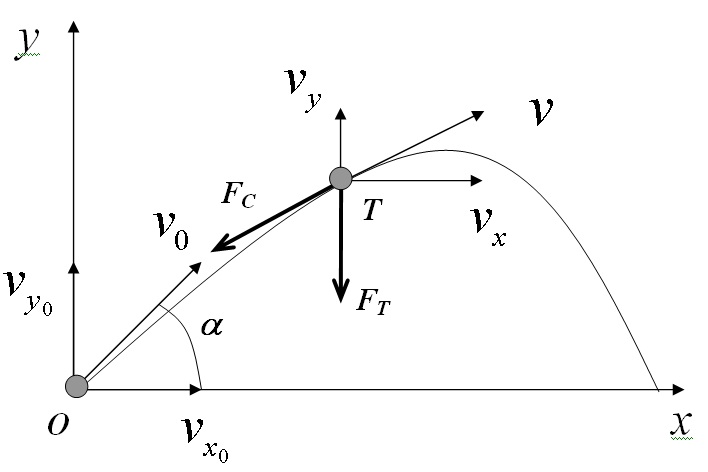
\includegraphics[width=1\linewidth]{img/newton_model.jpg}
	\caption{Модель Галилея\\(изображение с сайта rudn.ru).}
	\label{img:galilei_model}
\end{figure}

Модель Ньютона описывается системой уравнений, где координаты $x$, $y$ есть функции от $t$, где $t$ --- время.
В каждый момент скорости ее горизонтальная составляющая равна $v_x = v_0 \cos \alpha$, а вертикальная равна $v_y = v_0 \sin \alpha$.

В каждый момент времени координаты $x$, $y$ выражаются как
$$
\begin{cases}
x = (v_0 \cos \alpha) t, \\
y = (v_0 \sin \alpha) t - \frac{g t^2}{2},
\end{cases}
$$
где $g = 9.8$ м/с$^2$ --- ускорение свободного падения. Если выразить из первого уравнения системы $t$ через $x$ и подставив во второе уравнение, получим модель Галилея в следующем виде:
$$y = - \frac{g x^2}{2 v_0^2 \cos^2 \alpha} - x \tg \alpha.$$
Данное уравнение задает \textit{обратную задачу}, так как необходимо найти ненулевое расстояние по горизонтали $x$, при котором $y = 0$ (условие приземления тела).

\subsection{Модель Ньютона}
В модели Ньютона, в отличие от модели Галилея, учитывается сила сопротивления воздуха $F_с$, направленная противоположно вектору скорости $v$ и по модулю пропорциональная квадрату скорости $v^2$. Схема модели Ньютона приведена на рисунке~\ref{img:newton_model}.
\begin{figure}[h!]
	\centering
		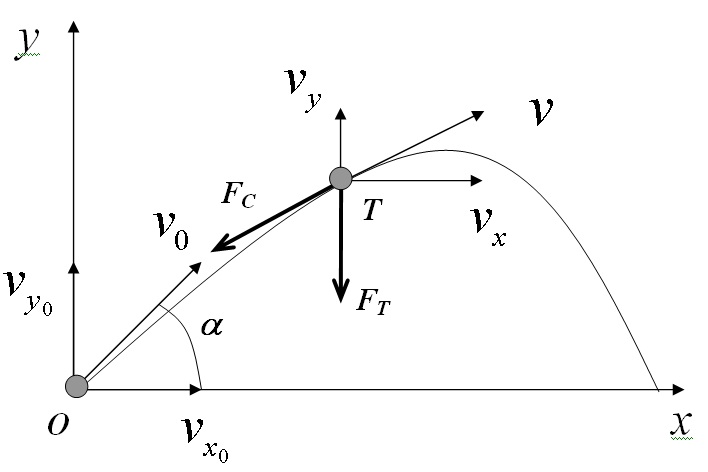
\includegraphics[width=1\linewidth]{img/newton_model.jpg}
	\caption{Модель Ньютона\\(изображение с сайта orenstudent.ru).}
	\label{img:newton_model}
\end{figure}

Сила сопротивления воздуха вычисляется по формуле $F_{\text с} = - \beta v^2$, $\beta = \frac{C \rho_{\text возд}S}{2}$, где $C$ --- баллистическая постоянная, $ C \approx 0,15$, $S$ --- площадь поперечного сечения снаряда, $\rho_{\text возд}$ --- плотность воздуха, $\rho_{\text возд} = 1,29 $ кг/м$^3$.
Обозначив координаты вектора скорости $v$ как $v_x = u$, $v_y = w$, запишем суммарное действие $F = (F_x, F_y)$ сил $F_{\text с}$ и $F_{\text т}$, действующие на снаряд в каждый момент времени ($F_{\text т}$ --- сила тяжести, $F_{\text т}=mg$):
$$
\begin{cases}
F_x = - \beta u \sqrt{u^2 + w^2}, \\
F_y = - \beta w \sqrt{u^2 + w^2} - mg,
\end{cases}
$$
 Откуда можно получить систему дифференциальных уравнений, описывающих движение тела:
\begin{equation}\label{eq:syst}
\left\{
\begin{array}{rcl}
m \cfrac{du}{dt} &=& - \beta u \sqrt{u^2 + w^2}, \\
m \cfrac{dw}{dt} &=& - \beta w \sqrt{u^2 + w^2} - mg, \\
\cfrac{dx}{dt} &=& u, \\
\cfrac{dy}{dt} &=& w.
\end{array}
\right.
\end{equation}
Получаем задачу Коши с начальными условиями:
 $$
 \left\{
\begin{array}{rcl}
u(0) &=& v_0 \cos \alpha, \\
w(0) &=& v_0 \sin \alpha, \\
x(0) &=& 0, \\
y(0) &=& 0.
\end{array}
\right.
$$

Полученная модель, описывающая движение тела, брошенного под углом к горизонту с учетом силы сопротивления воздухе, является моделью Ньютона. Можно показать, что при $\beta = 0$ модель Ньютона совпадает с моделью Галилея.

Система~\ref{eq:syst} не решается аналитически и требует численных методов решения систем дифференциальных уравнений, таких как метод Рунге-Кутты четвертого порядка.
\section{Текст программы}
Для сравнения моделей Галилея и Ньютона была написана программа, рисующая графики движения тела, брошенного под углом к горизонту и вычисляющая координаты точек падения для каждого метода.
Программа реализована на языке Python, решение системы~\ref{eq:syst} выполняется функцией {\ttfamily solve\_ivp} модуля {\ttfamily scipy.integrate}. Массивы решений для $x$ и $y$ {\ttfamily coords} отрисовываются на экране с помощью функции {\ttfamily plot} модуля {\ttfamily matplotlib.pyplot}. Для каждого момента времени $t$ из массива {\ttfamily t\_arr}, вычисляем соотвутствующие координаты $x$ и $y$, используя модель Галилея, полученные массивы точек {\ttfamily gal\_xval} и {\ttfamily gal\_yval} так же отрисовываются на том же графике.
\begin{figure}[H]
\begin{lstlisting}[language=python, caption={Вычисление параметров системы~\ref{eq:syst}.},label={lst:init_params}]
rho_lead = 11340  # kg/m^3
rho_air = 1.29    # kg/m^3
d = 0.1  # m
alpha = pi / 4  # angle, radians
v0 = 200         # start velocity
t_0   = 0       # time limits, sec
t_max = 100
eps = 1.e-2

r = d/2
V = (4/3) * pi*(r**3)  # volume
m = rho_lead * V
C = 0.15  # ballistic constant
# C = 0
S = pi * (r**2)
beta = C * rho_air * S / 2
g = 9.8  # m/sec^2
\end{lstlisting}
\end{figure}
\begin{figure}[H]
\begin{lstlisting}[language=python, caption={Решение системы дифференциальных уравнений, описывающих движение тела в модели Ньютона.},label={lst:dif_eq_solution}]
## Функция, реализующая правые части системы
def f(t, system):
    (u, w, x, y) = system
    root = math.sqrt(u**2 + w**2)
    factor = -beta*root/m
    return np.ndarray((4,), buffer=np.array([u*factor, w*factor-g, u, w]))

## Начальные условия
u0 = v0*math.cos(alpha)
w0 = v0*math.sin(alpha)
x0 = 0
y0 = 0

## Функция, отбрасывающая точки правее точки приземления
def trim(arr):
    M = np.where(arr[1] >= 0)[-1][-1]
    return arr[:M, :M]
    
t_arr = coords['t']  # Массив точек t
system0 = np.ndarray((4,), buffer=np.array([u0, w0, x0, y0]))
coords = solve_ivp(f, (t_0, t_max), system0, max_step=eps)
\end{lstlisting}
\end{figure}
\begin{figure}[H]
\begin{lstlisting}[language=python, caption={Вычисление координат снаряда в каждый момент времени в модели Галилея.},label={lst:galilei_solution}]
def Galilei_x(t):
    return v0*math.cos(alpha)*t
    
def Galilei_y(t):
    return v0*math.sin(alpha)*t-g*(t**2)/2

gal_xvals = [Galilei_x(t) for t in t_arr] # t_arr --- массив точек t
gal_yvals = [Galilei_y(t) for t in t_arr]
\end{lstlisting}
\end{figure}
\section{Тесты}
\subsection{Начальная скорость 200\,м/с}
Возьмем $\alpha = \dfrac{\pi}{4}$, $v_0 = 200$м/с. Сопротивление воздуха в модели Ньютона учитывается. Максимальный шаг $\Delta t=1.e-2$.

Результат работы программы представлен на рисунке~\ref{img:1_a-45_v-200}.\\
Координаты точки падения тела в модели Ньютона: $(x_N, y_N) = (2952.89, 2.06)$. \\
Координаты точки падения тела в модели Галилея: $(x_G, y_G) = (4079.70, 1.93)$.

Отличие результатов дальности полета в модели Галилея и в модели Ньютона составляет $|1-\frac{x_G}{x_N}| \times 100\% = 38\% $.
\begin{figure}[h!]
	\centering
		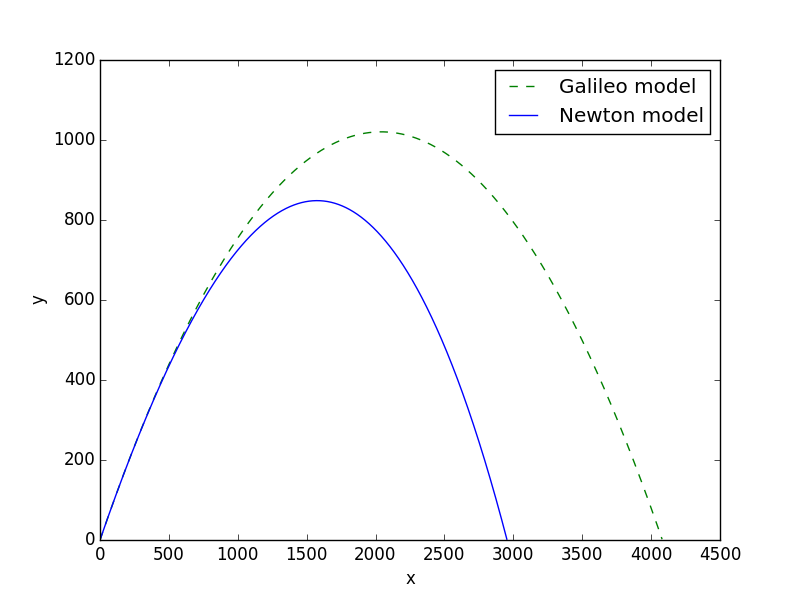
\includegraphics[width=1\linewidth]{img/1_a-45_v-200.png}
	\caption{Моделирование полета тела, брошенного под углом к горизонту, $\alpha = \dfrac{\pi}{4}$, $v_0 = 200\,$м/с, сопротивление воздуха учитывается.}
	\label{img:1_a-45_v-200}
\end{figure}

Результат работы программы в случае, когда коэффициент $\beta$ равен нулю (сопротивление воздуха не учитывается) представлен на рисунке~\ref{img:2_a-45_v-200}.\\
Координаты точки падения тела в модели Ньютона: $(x_N, y_N) = (4079.70, 1.93)$. \\
Координаты точки падения тела в модели Галилея: $(x_G, y_G) = (4079.70, 1.93)$.
\begin{figure}[h!]
	\centering
		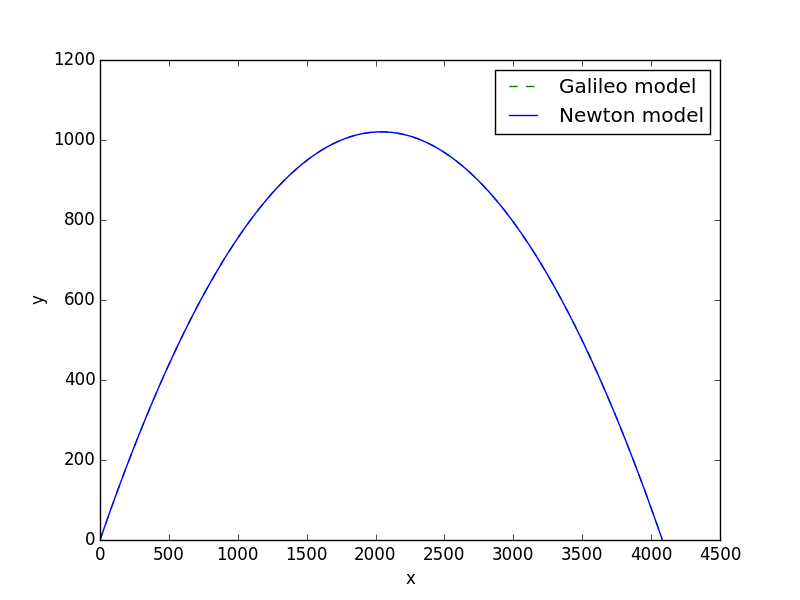
\includegraphics[width=1\linewidth]{img/2_a-45_v-200.png}
	\caption{Моделирование полета тела, брошенного под углом к горизонту, $\alpha = \dfrac{\pi}{4}$, $v_0 = 200\,$м/с, сопротивление воздуха не учитывается.}
	\label{img:2_a-45_v-200}
\end{figure}

Как видно из результатов тестов, расстояние, которое пролетает тело в модели Галилея и в модели Ньютона совпадают в условиях отсутствия сопротивления воздуха.

\subsection{Начальная скорость 50\,м/с}
Возьмем $\alpha = \dfrac{\pi}{4}$, $v_0 = 200$м/с. Сопротивление воздуха в модели Ньютона учитывается. Максимальный шаг $\Delta t=1.e-2$.

Результат работы программы представлен на рисунке~\ref{img:1_a-45_v-50}.\\
Координаты точки падения тела в модели Ньютона: $(x_N, y_N) = (248.31, 0.47)$. \\
Координаты точки падения тела в модели Галилея: $(x_G, y_G) = (254.67, 0.43)$.

Отличие результатов дальности полета в модели Галилея и в модели Ньютона составляет $|1-\frac{x_G}{x_N}| \times 100\% = 2,4\% $
\begin{figure}[h!]
	\centering
		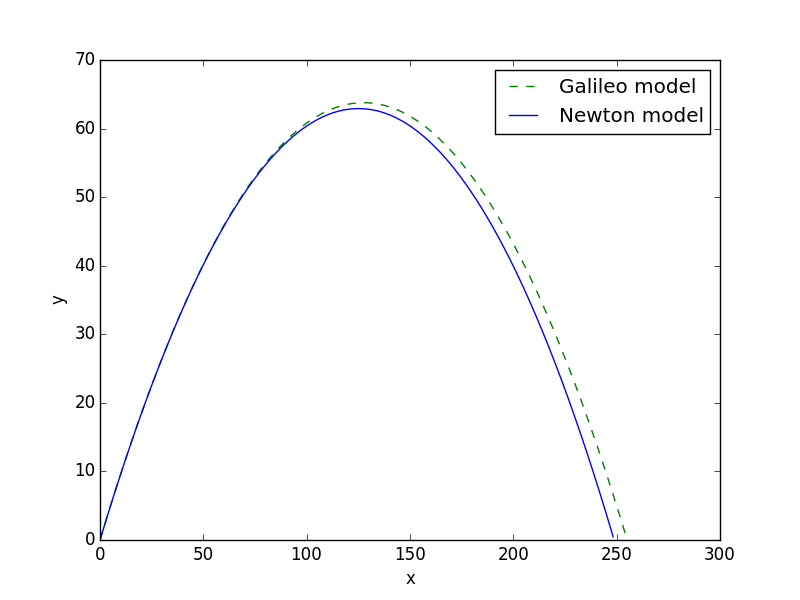
\includegraphics[width=1\linewidth]{img/1_a-45_v-50.png}
	\caption{Моделирование полета тела, брошенного под углом к горизонту, $\alpha = \dfrac{\pi}{4}$, $v_0 = 50\,$м/с, сопротивление воздуха учитывается.}
	\label{img:1_a-45_v-50}
\end{figure}
\subsection{Начальная скорость 5\,м/с}
Возьмем $\alpha = \dfrac{\pi}{4}$, $v_0 = 200$м/с. Сопротивление воздуха в модели Ньютона учитывается. Максимальный шаг $\Delta t=1.e-3$.

Результат работы программы представлен на рисунке~\ref{img:1_a-45_v-5}.\\
Координаты точки падения тела в модели Ньютона: $(x_N, y_N) = (2.546, 0.004)$. \\
Координаты точки падения тела в модели Галилея: $(x_G, y_G) = (2.547, 0.004)$.

Отличие результатов дальности полета в модели Галилея и в модели Ньютона составляет $|1-\frac{x_G}{x_N}| \times 100\% = 0,04\% $
\begin{figure}[h!]
	\centering
		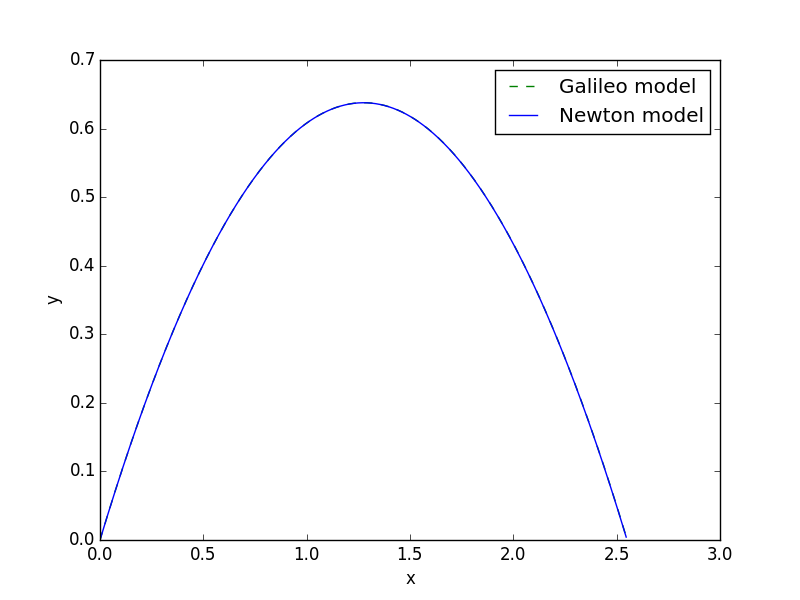
\includegraphics[width=1\linewidth]{img/1_a-45_v-5.png}
	\caption{Моделирование полета тела, брошенного под углом к горизонту, $\alpha = \dfrac{\pi}{4}$, $v_0 = 5\,$м/с, сопротивление воздуха учитывается.}
	\label{img:1_a-45_v-5}
\end{figure}
%
\anonsection{Заключение}
По результатам проведенных тестов можно сделать вывод, что дальность падения снаряда, брошенного под углом к горизонту, для моделей Галилея и Ньютона отличается тем больше, чем больше начальная скорость (для дальности полета в несколько километров разница составила больше 1\,км, для дальности полета в двести метров --- разница в несколько метров, при дальности полета в несколько метров отличия практически не заметны).

Таким образом, модель Галилея применима для бросания снаряда на небольшие расстояния. При увеличении дальности полета влияние силы сопротивления воздуха становится достаточно значительным, и им уже нельзя принебречь.

При еще больших расстояниях становится необходимо учитывать и кривизну поверхности Земли, и изменение ускорения свободного падения~$g$, и момент вращения снаряда, поэтому модель Ньютона также становится неприменимой.
\end{document}